\documentclass{beamer}
\usepackage{animate}
\usepackage{tikz}
\usepackage[style=authoryear-comp, backend=biber]{biblatex}
\usepackage{caption}
\usepackage{datetime}

% https://ctan.mirror.garr.it/mirrors/ctan/macros/latex/contrib/beamer-contrib/themes/beamertheme-gotham/gotham.pdf
\usetheme{gotham}
\gothamset{
partframe default=off,
sectionframe default=on,
sectiontocframe default=off,
}

% \setlength{\footskip}{5cm}

\renewcommand*{\bibfont}{\tiny}
\addbibresource{bib.bib}

\title{Illusioni di Intelligenza e Comportamenti emergenti}
\subtitle{Limiti e Potenzialità degli LLM}
\author{Nicolò Vescera}
\date{10/04/2025}

\begin{document}

\begin{frame}
    \titlepage
    \begin{tikzpicture}[remember picture, overlay]
        \node[left=1cm] at (current page.-20) 
        {
            
\includegraphics[width=2cm]{imgs/unipg/unipg_logo.png}
        };
        \node[right=1cm] at (current page.200) 
        {
            
\includegraphics[width=2cm]{imgs/unipg/dmi_logo.png}
        };
        \end{tikzpicture}
\end{frame}

\begin{frame}{Outline}
    \tableofcontents
\end{frame}

\section{Definizione ed esempi di IA}

\begin{frame}{Cos'è l'IA?}
    \pause
    L’IA è un \textbf{settore dell’Informatica} che tenta di \textbf{creare macchine} con caratteristiche tipiche dell’\textbf{intelligenza umana}.
\end{frame}

\begin{frame}{L'IA intorno a noi}
    \begin{figure}
        \centering
        
\includegraphics[width=.4\linewidth]{imgs/rec_system/amazon_recsys.png}
        
\includegraphics[width=.4\linewidth]{imgs/rec_system/primevideo_recsys.png}
        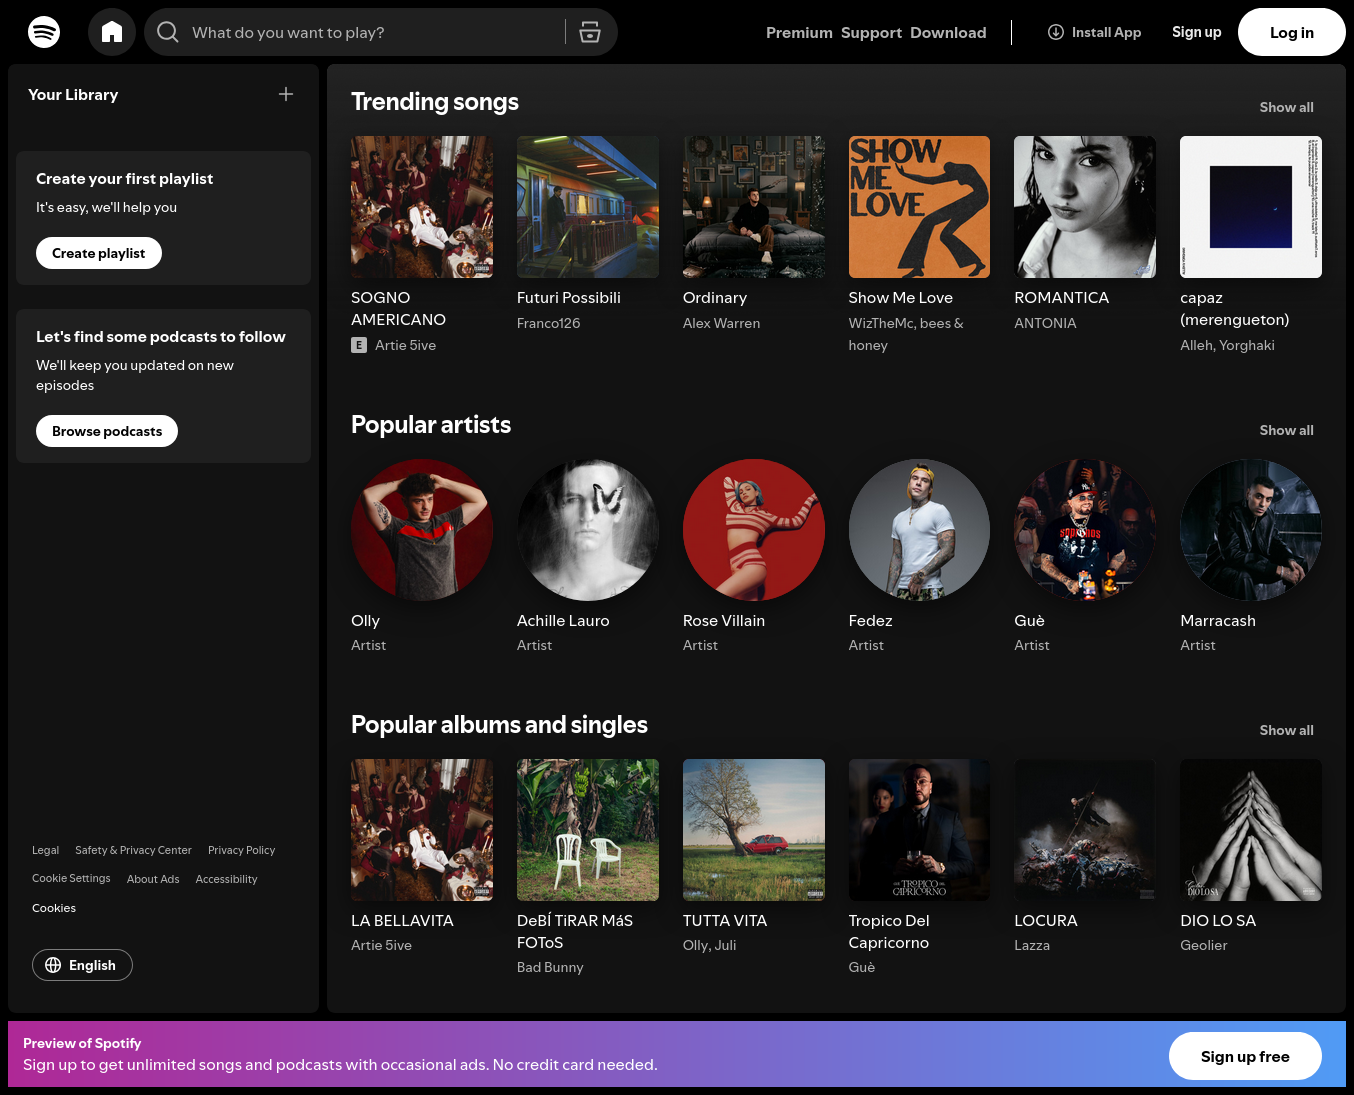
\includegraphics[width=.4\linewidth]{imgs/rec_system/spotify_recsys.png}
    \end{figure}
\end{frame}

\begin{frame}{L'IA intorno a noi}
    \begin{figure}
        \centering
        \animategraphics[autoplay,loop,width=\linewidth]{5}{anims/auto/frame-}{1}{39}
        \caption*{\textcolor{gray}{Geopop: https://youtu.be/-D2kPFkwTmg}}
    \end{figure}
\end{frame}

\begin{frame}{L'IA intorno a noi}
    \begin{figure}
        \centering
        \animategraphics[autoplay,loop,width=\linewidth]{10}{anims/zebra/frame-}{1}{62}
        \caption*{\textcolor{gray}{CycleGAN (2017)\\https://youtu.be/9reHvktowLY}}
    \end{figure}
\end{frame}

\begin{frame}{L'IA intorno a noi}
    \begin{figure}
        \centering
        \animategraphics[autoplay,loop,width=\linewidth]{10}{anims/deepfake/frame-}{1}{79}
        \caption*{\textcolor{gray}{Geopop: https://youtu.be/AfUKFhowdNc}}
    \end{figure}
\end{frame}

\begin{frame}{L'IA intorno a noi}
    \begin{figure}
        \centering
        
\includegraphics[width=.4\linewidth]{imgs/llms_logo/chatgpt_logo.jpg}
        
\includegraphics[width=.4\linewidth]{imgs/llms_logo/deepseek_logo.png}
        
\includegraphics[width=.4\linewidth]{imgs/llms_logo/copilot_logo.png}
    \end{figure}
\end{frame}

\section{Storia}
\begin{frame}{Chi ha inventato l'IA?}
    \begin{columns}[T]
    \begin{column}{.48\textwidth}
        \textbf{Alan Turing} (1912-1954)
        
        \begin{itemize}
            \item Matematico inglese
            \item Viene considerato il padre dell'Informatica
            \item Decifrò il codice Enigma
            \item Inventore della macchina di Turing
        \end{itemize}
    \end{column}

    \hfill
    
    \begin{column}{.48\textwidth}
        \begin{figure}
            \centering
            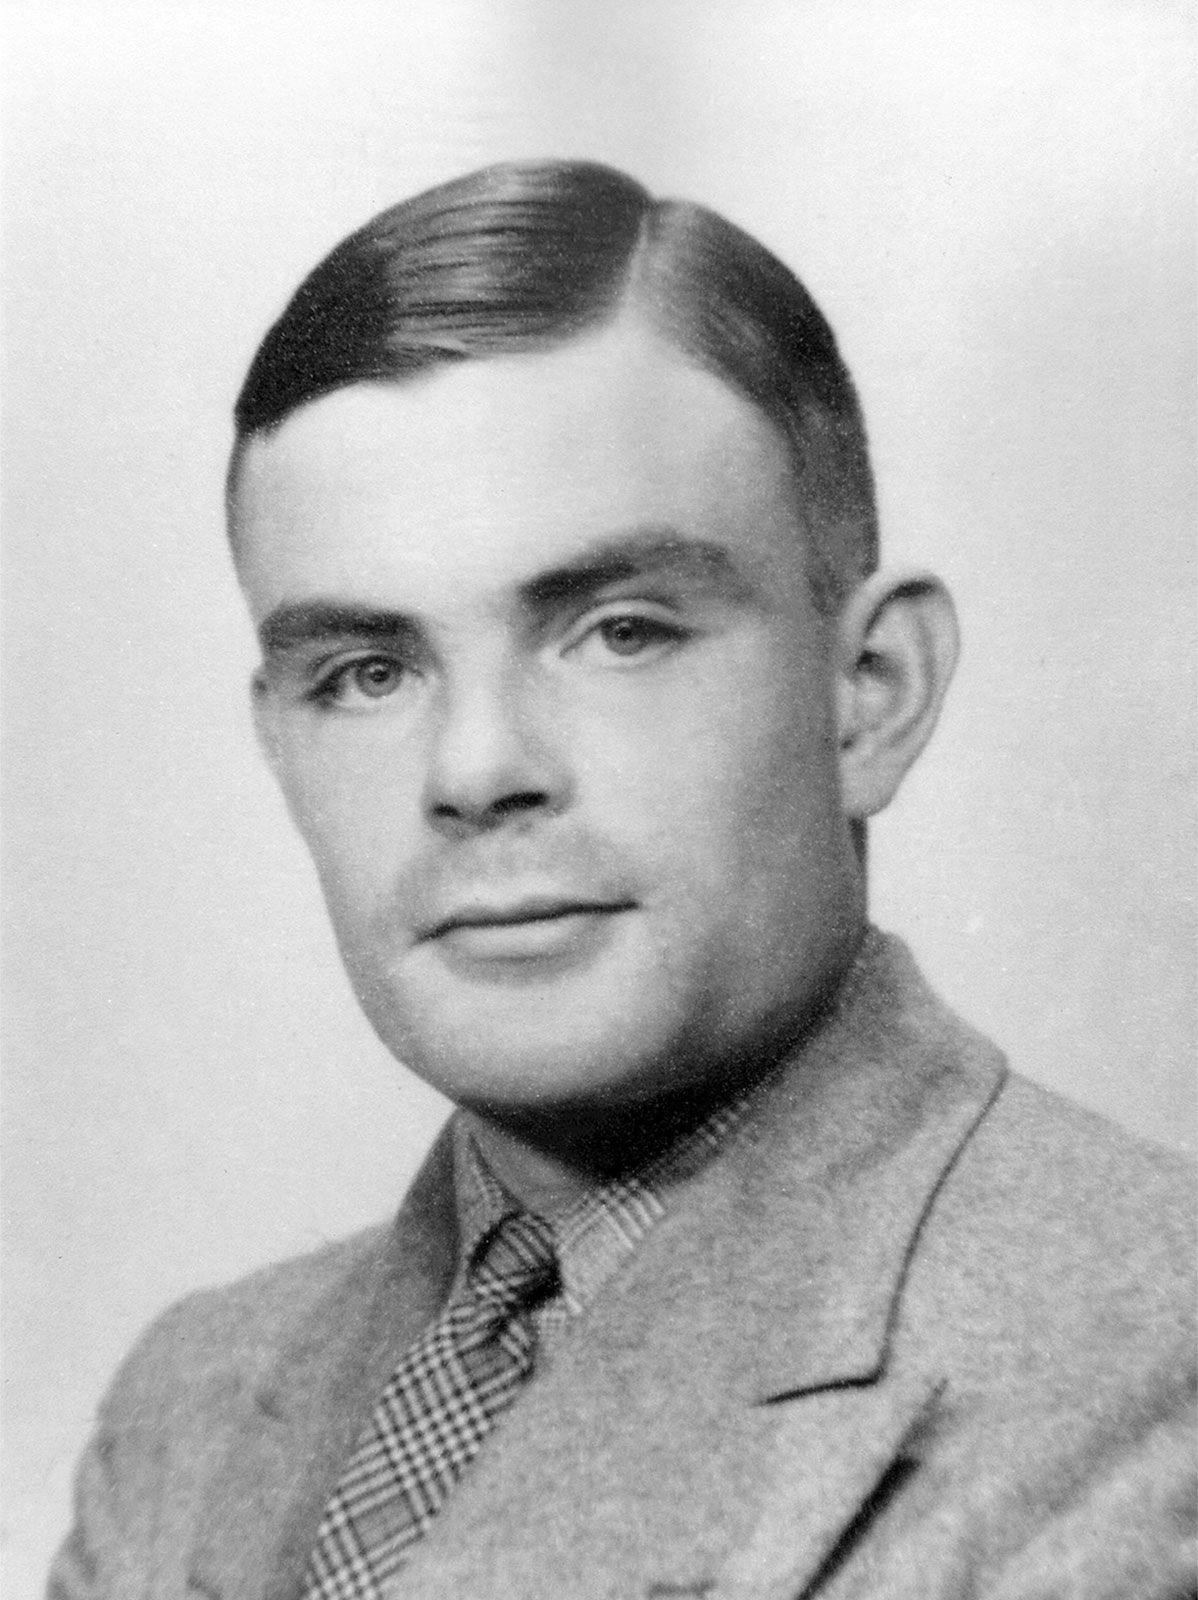
\includegraphics[width=.9\linewidth]{imgs/turing.jpg}
        \end{figure}
    \end{column}
    \end{columns}
\end{frame}

\begin{frame}{The Imitation Game}
    \begin{figure}
        \centering
        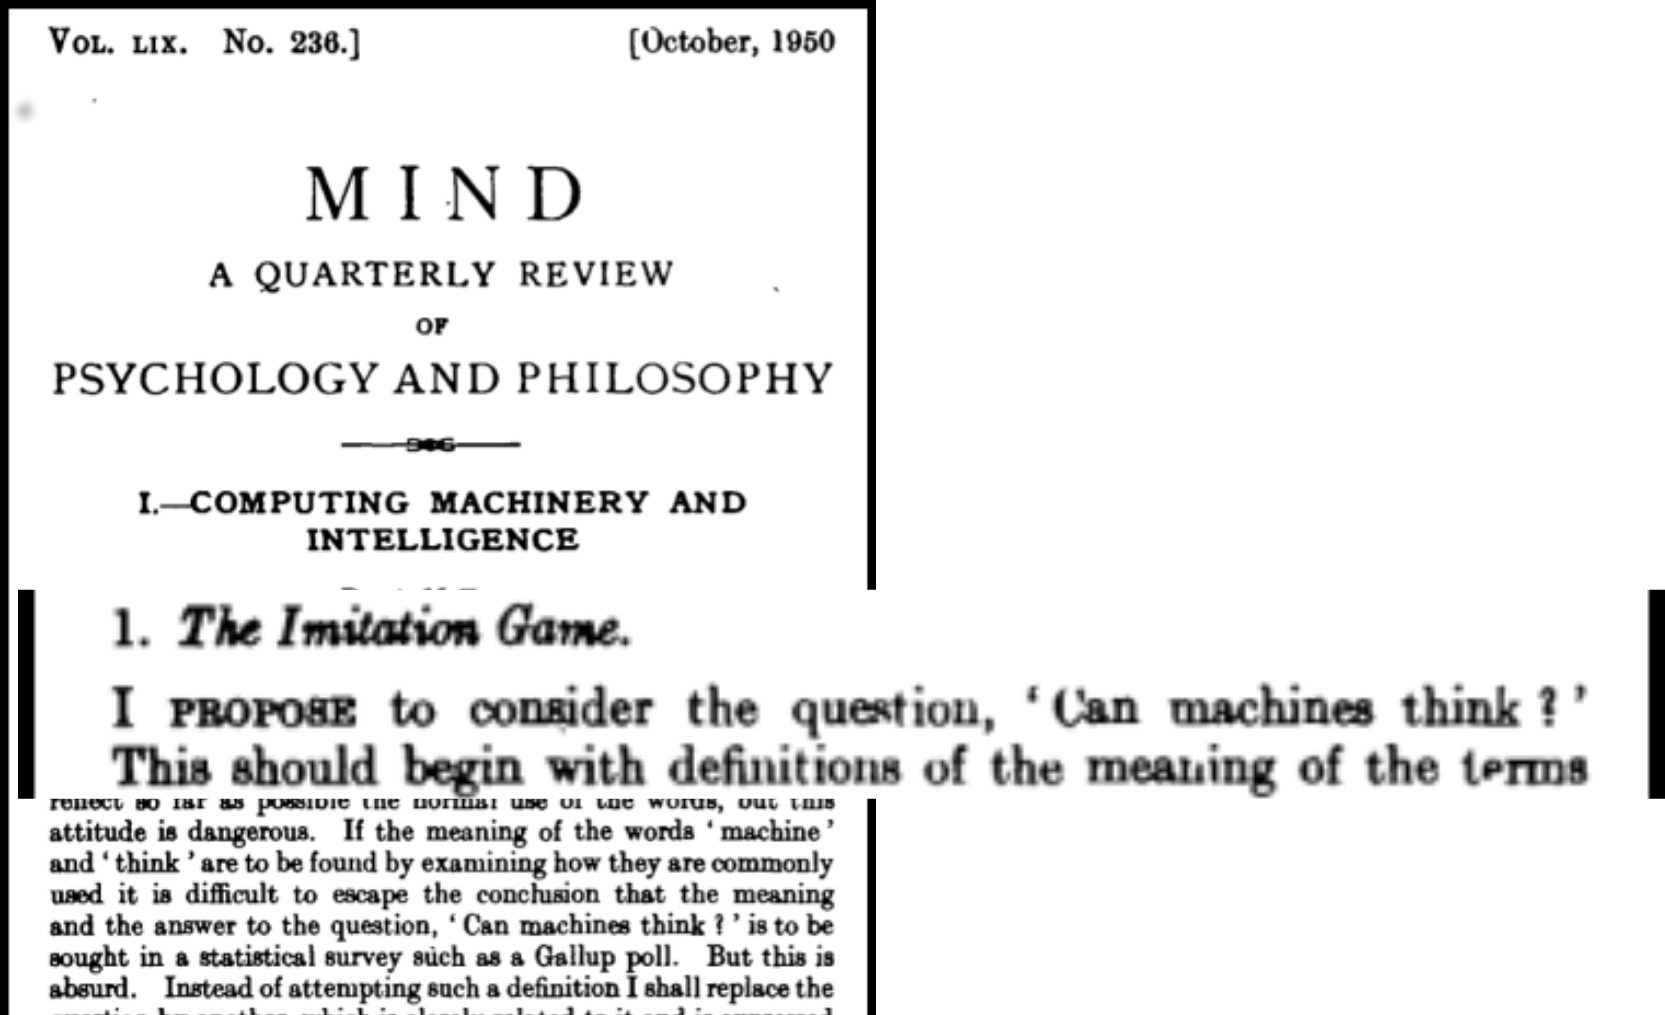
\includegraphics[width=0.9\linewidth]{imgs/AI-Sviluppi-Sfide-Opportunita.png}
    \end{figure}
\end{frame}

\begin{frame}{The Imitation Game}
    \begin{figure}
        \centering
        \animategraphics[autoplay,loop,width=.5\linewidth]{10}{anims/turing/frame-}{1}{127}
    \end{figure}
\end{frame}

\begin{frame}{Definizione di Intelligenza}
Complesso di facoltà psichiche e mentali che consentono all’uomo di pensare, comprendere o spiegare i fatti o le azioni, elaborare modelli astratti della realtà, intendere e farsi intendere dagli altri, giudicare, e lo rendono insieme capace di adattarsi a situazioni nuove e di modificare la situazione stessa quando questa presenta ostacoli all’adattamento; propria dell’uomo, [...]\footnote[1]{Treccani online, "Intellig\`enza"\\ \ \\}
\end{frame}

\begin{frame}{Definizione di Intelligenza}
Complesso di facoltà psichiche e mentali che consentono all’uomo di pensare, \textcolor{red}{\textbf{comprendere}} o spiegare i fatti o le azioni, elaborare modelli astratti della realtà, intendere e farsi intendere dagli altri, giudicare, e lo rendono insieme capace di adattarsi a situazioni nuove e di modificare la situazione stessa quando questa presenta ostacoli all’adattamento; propria dell’uomo, [...]\footnote[1]{Treccani online, "Intellig\`enza"\\ \ \\}
\end{frame}

\begin{frame}{Definizione di Intelligenza}
Complesso di facoltà psichiche e mentali che consentono all’uomo di pensare, \textcolor{red}{\textbf{comprendere}} o spiegare i fatti o le azioni, \textcolor{red}{\textbf{elaborare}} modelli astratti della realtà, intendere e farsi intendere dagli altri, giudicare, e lo rendono insieme capace di adattarsi a situazioni nuove e di modificare la situazione stessa quando questa presenta ostacoli all’adattamento; propria dell’uomo, [...]\footnote[1]{Treccani online, "Intellig\`enza"\\ \ \\}
\end{frame}

\begin{frame}{Definizione di Intelligenza}
Complesso di facoltà psichiche e mentali che consentono all’uomo di pensare, \textcolor{red}{\textbf{comprendere}} o spiegare i fatti o le azioni, \textcolor{red}{\textbf{elaborare}} modelli astratti della realtà, intendere e farsi intendere dagli altri, giudicare, e lo rendono insieme capace di \textcolor{red}{\textbf{adattarsi}} a situazioni nuove e di modificare la situazione stessa quando questa presenta ostacoli all’adattamento; propria dell’uomo, [...]\footnote[1]{Treccani online, "Intellig\`enza"\\ \ \\}
\end{frame}

\begin{frame}{Definizione di Intelligenza}
Complesso di facoltà psichiche e mentali che consentono all’uomo di pensare, \textcolor{red}{\textbf{comprendere}} o spiegare i fatti o le azioni, \textcolor{red}{\textbf{elaborare}} modelli astratti della realtà, intendere e farsi intendere dagli altri, \colorbox{yellow!70}{\textcolor{red}{\textbf{giudicare}}}, e lo rendono insieme capace di \textcolor{red}{\textbf{adattarsi}} a situazioni nuove e di modificare la situazione stessa quando questa presenta ostacoli all’adattamento; propria dell’uomo, [...]\footnote[1]{Treccani online, "Intellig\`enza"\\ \ \\}
\end{frame}

\section{Ma quindi l'IA è intelligente ?}

\begin{frame}{Ma quindi l'IA è intelligente ?}
    \begin{center}
        \begin{tikzpicture}
          \node (img1) {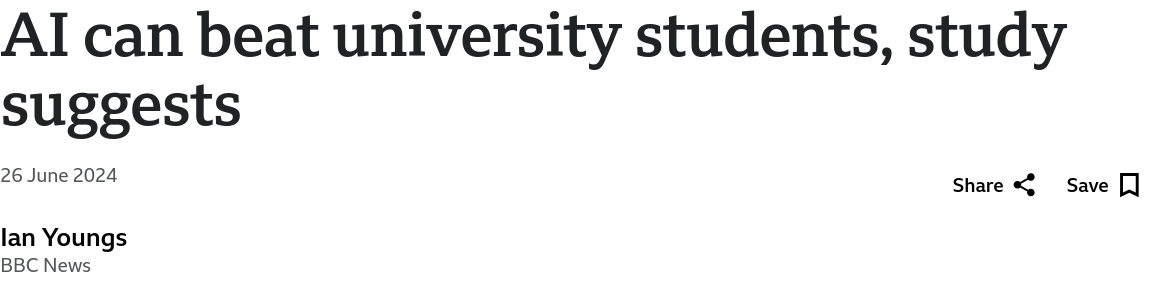
\includegraphics[width=.8\linewidth]{imgs/ai-vs-uni/ai_vs_uni_2.png}};
          \node (img4) at (img1.south west) [xshift=0.8cm, yshift=-0.8cm] {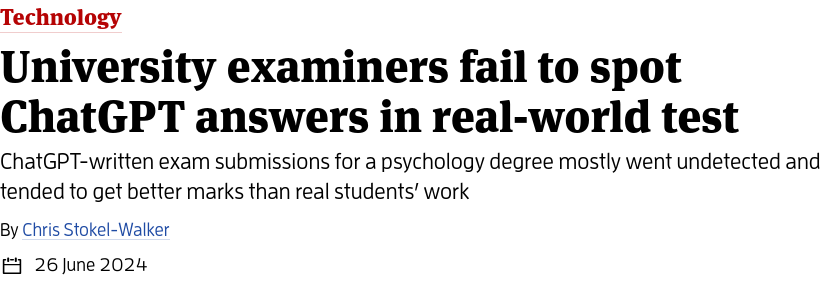
\includegraphics[width=.4\linewidth]{imgs/ai-vs-uni/chatgpt_vs_uni.png}};
          \node (img2) at (img1.south east) [xshift=-2.5cm, yshift=0.5cm] {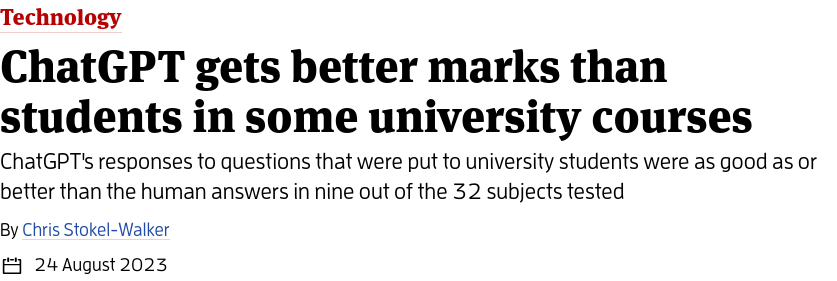
\includegraphics[width=.6\linewidth]{imgs/ai-vs-uni/ai_vs_uni.png}};
          \node (img3) at (img1.north west) [xshift=3cm, yshift=1cm] {
\includegraphics[width=.6\linewidth]{imgs/ai-vs-uni/ai_vs_uni_3.png}};
        \end{tikzpicture}
    \end{center}
\end{frame}

\begin{frame}{Come funziona ChatGPT ?}
    \begin{figure}
        \centering
        \animategraphics[autoplay,loop,width=.9\linewidth]{10}{anims/gpt/frame-}{1}{199}
        \caption*{\textcolor{gray}{3Blue1Brown: https://youtu.be/wjZofJX0v4M}}
    \end{figure}
\end{frame}

\begin{frame}{Funzionamento}
    \begin{figure}
        \centering
        \animategraphics[autoplay,loop,width=.9\linewidth]{10}{anims/gptres/frame-}{1}{299}
        \caption*{\textcolor{gray}{3Blue1Brown: https://youtu.be/wjZofJX0v4M}}
    \end{figure}
\end{frame}

\begin{frame}{Embedding}
    \begin{figure}
        \centering
        \animategraphics[autoplay,loop,width=.9\linewidth]{10}{anims/wembedd/frame-}{1}{218}
        \caption*{\textcolor{gray}{3Blue1Brown: https://youtu.be/wjZofJX0v4M}}
    \end{figure}
\end{frame}

\begin{frame}{Embedding}
    \begin{figure}
        \centering
        \animategraphics[autoplay,loop,width=.9\linewidth]{10}{anims/gptembedding/frame-}{1}{94}
        \caption*{\textcolor{gray}{3Blue1Brown: https://youtu.be/wjZofJX0v4M}}
    \end{figure}
\end{frame}

\begin{frame}{Embedding}
    \begin{figure}
        \centering
        \animategraphics[autoplay,loop,width=.9\linewidth]{10}{anims/gptvectors/frame-}{1}{269}
        \caption*{\textcolor{gray}{3Blue1Brown: https://youtu.be/wjZofJX0v4M}}
    \end{figure}
\end{frame}

\begin{frame}{Stochastic Parrots}
    \begin{figure}
        
\includegraphics[width=.7\linewidth]{imgs/parrot/parrot.png}
    \end{figure}
\end{frame}

\begin{frame}{Stochastic Parrots}
    \begin{figure}
        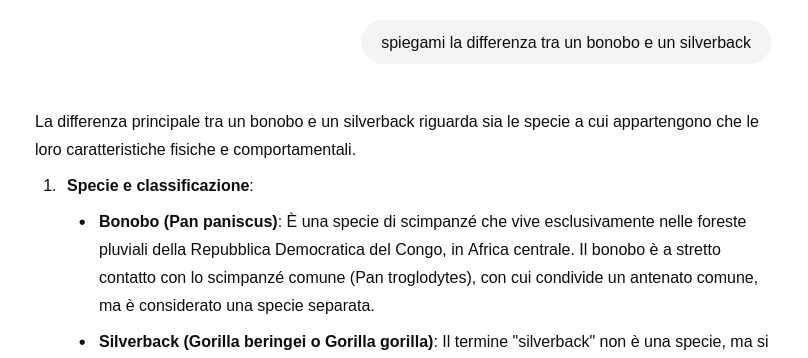
\includegraphics[width=1.0\linewidth]{imgs/parrot/gpt_gorilla.png}
    \end{figure}
    
\end{frame}
\begin{frame}{Stochastic Parrots}
    \begin{figure}
        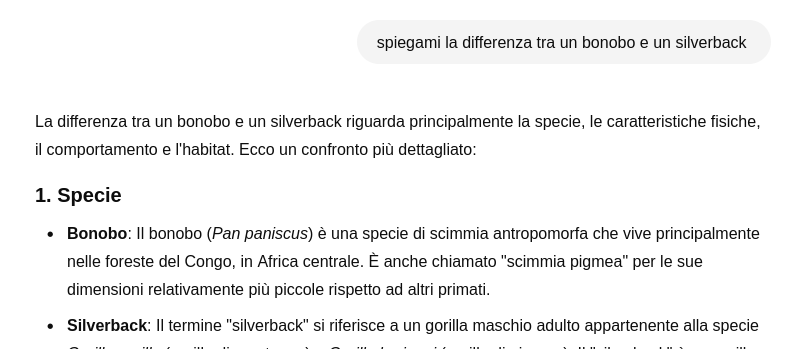
\includegraphics[width=1.0\linewidth]{imgs/parrot/gpt_gorilla2.png}
    \end{figure}
\end{frame}

\begin{frame}{Stochastic Parrots}
    \begin{figure}
        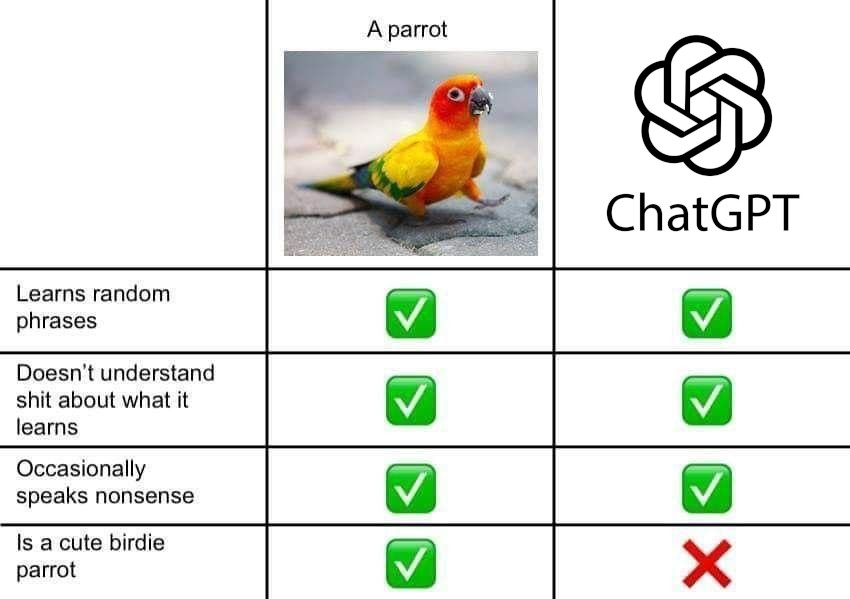
\includegraphics[width=.8\linewidth]{imgs/parrot/gpt_vs_parrot2.jpg}
    \end{figure}
\end{frame}

\begin{frame}{Allucinazioni}
    \begin{figure}
        \centering
        
\includegraphics[width=1.0\linewidth]{imgs/chatgpt_all_2.png}
    \end{figure}
\end{frame}

\section{Il fenomeno dei Comportamenti emergenti}

\begin{frame}{Definizione}
  \textit{``Un'abilit\`a viene definita emergente se \`e presente in modelli di pi\`u grandi dimensioni, ma non in quelli di dimensioni pi\`u piccole.''}\footnote{Emergent Abilities of Large Language Models\\ \ \\}
\end{frame}

\begin{frame}{Comportamenti emergenti: Traduzione}
    \begin{figure}
        \centering
        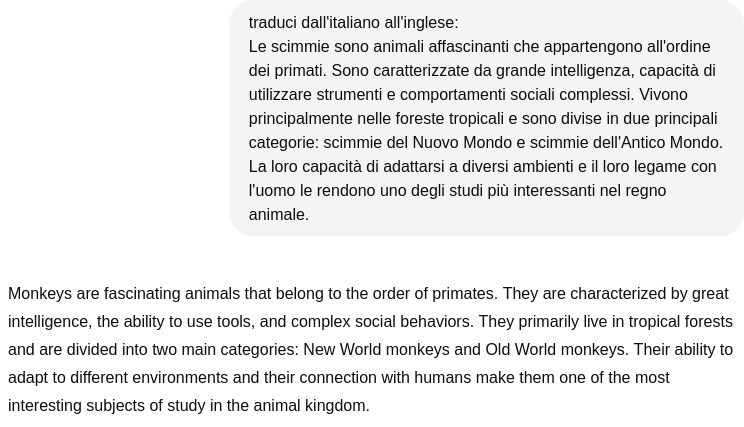
\includegraphics[width=.8\linewidth]{imgs/emergent/gpt_monkey2.png}
    \end{figure}
\end{frame}

\begin{frame}{Comportamenti emergenti: Coding}
    \begin{figure}
        \centering
        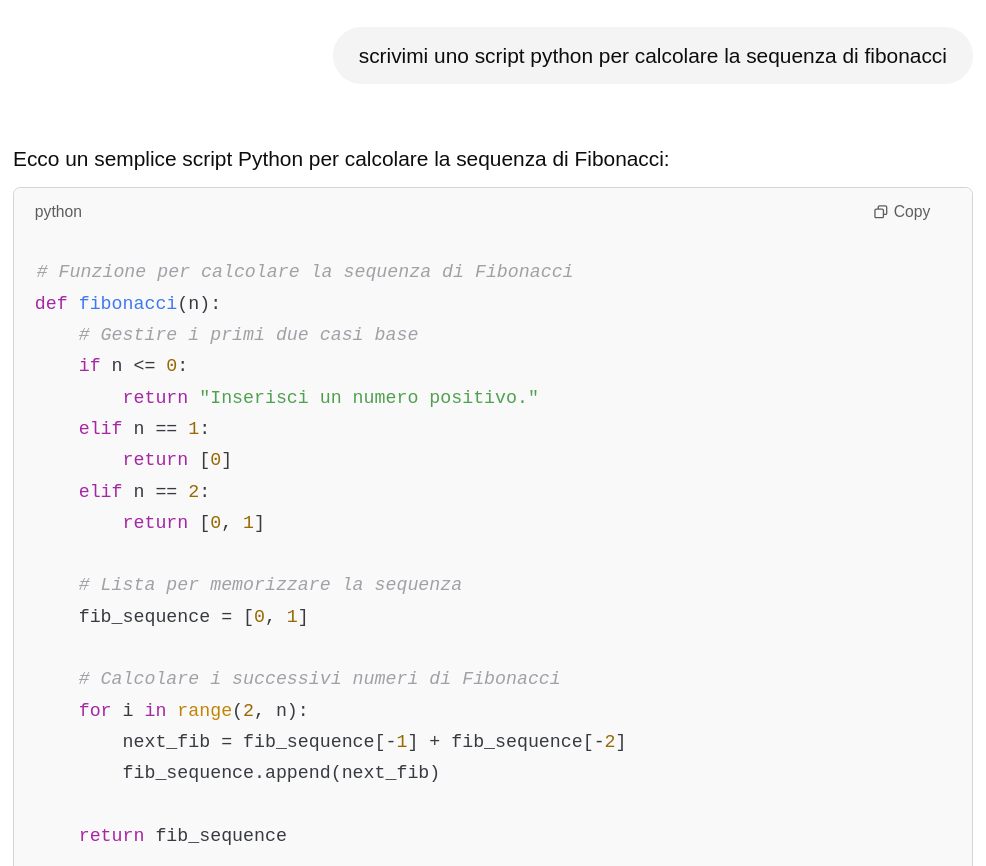
\includegraphics[width=.8\linewidth]{imgs/emergent/gpt_fibonacci2.png}
    \end{figure}
\end{frame}

\begin{frame}{Comportamenti emergenti}
    \begin{figure}
        \centering
        \caption*{\textbf{Dipendono dalle dimensioni del modello}}
        \animategraphics[autoplay,loop,width=.8\linewidth]{10}{anims/gptalbero/frame-}{1}{64}
    \end{figure}
\end{frame}

\begin{frame}{Dimensione del modello}
    \begin{figure}
        \centering
        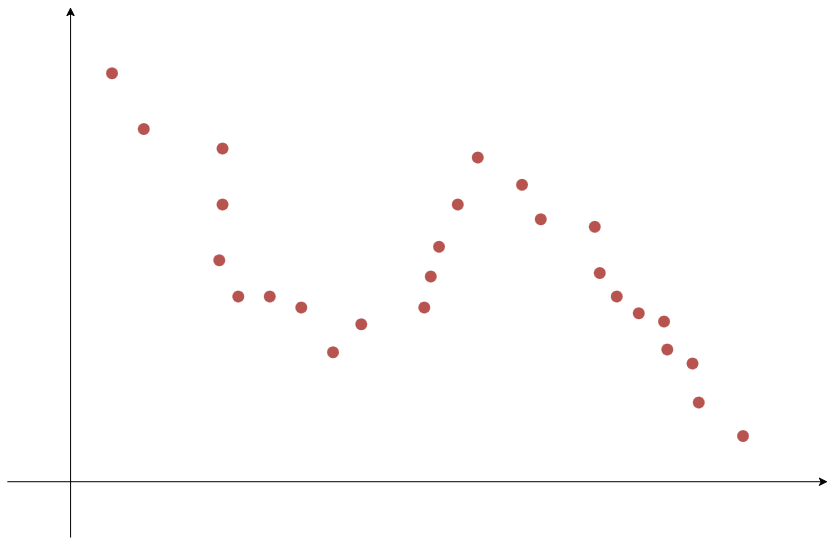
\includegraphics[width=.7\linewidth]{imgs/emergent/chartnninitial.png}
        \caption*{Vogliamo trovare una funzione che approssimi questi dati}
    \end{figure}
\end{frame}

\begin{frame}{Dimensione del modello}
    \begin{figure}
        \centering
        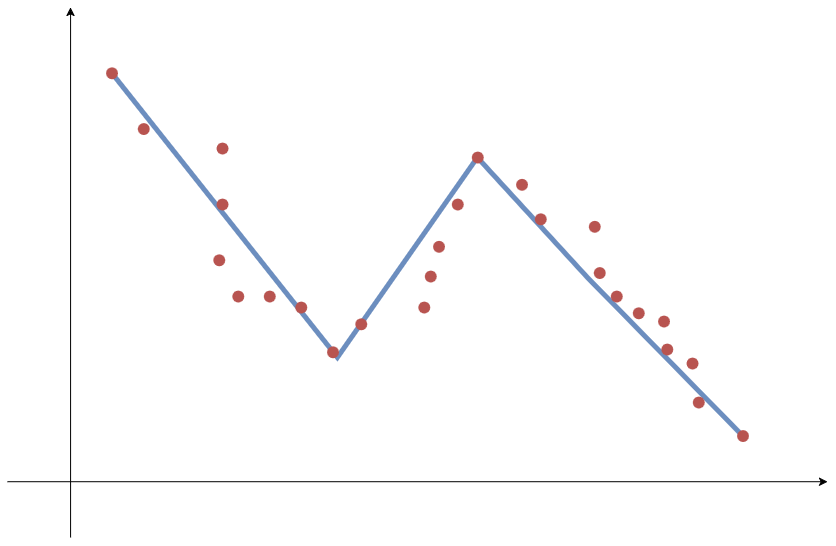
\includegraphics[width=.7\linewidth]{imgs/emergent/chartnn.badbad.png}
        \caption*{Con un Modello con Pochi parametri}
    \end{figure}
\end{frame}

\begin{frame}{Dimensione del modello}
  \begin{columns}
    \begin{column}{0.48\textwidth}
        \begin{figure}
            \centering
            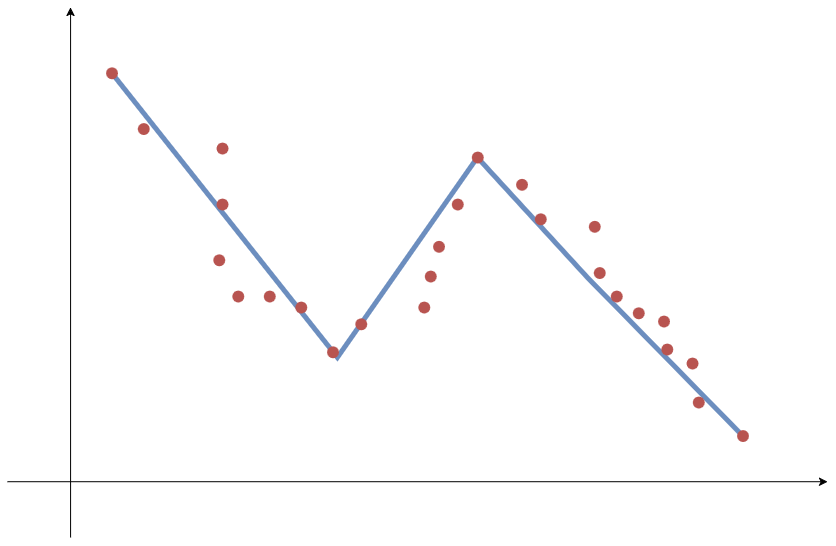
\includegraphics[width=1.0\linewidth]{imgs/emergent/chartnn.badbad.png}
            \caption*{Pochi parametri}
        \end{figure}
    \end{column}
    
    \begin{column}{0.48\textwidth}
        \begin{figure}
            \centering
            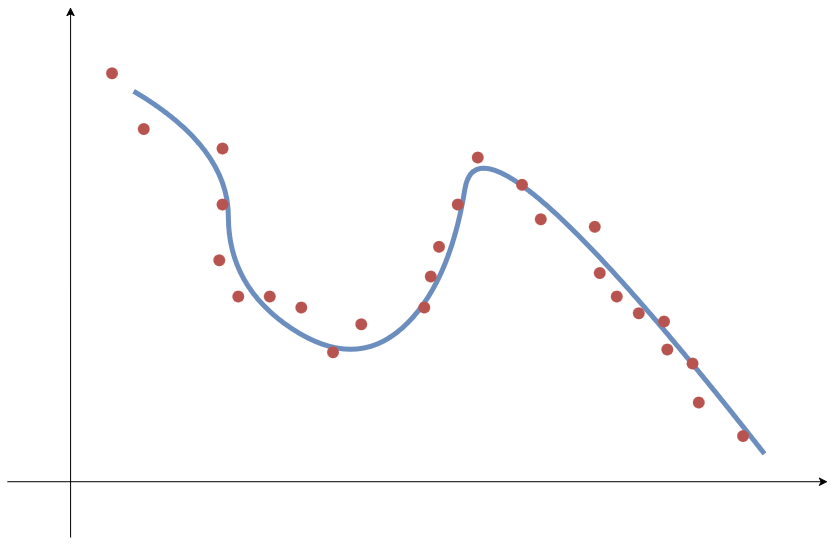
\includegraphics[width=1.0\linewidth]{imgs/emergent/chartnngoodgrosso(1).png}
            \caption*{Molti parametri}
        \end{figure}
    \end{column}
  \end{columns}
\end{frame}

\begin{frame}{Dimensione del modello}
  \begin{columns}
    \begin{column}{0.48\textwidth}
        \begin{figure}
            \centering
            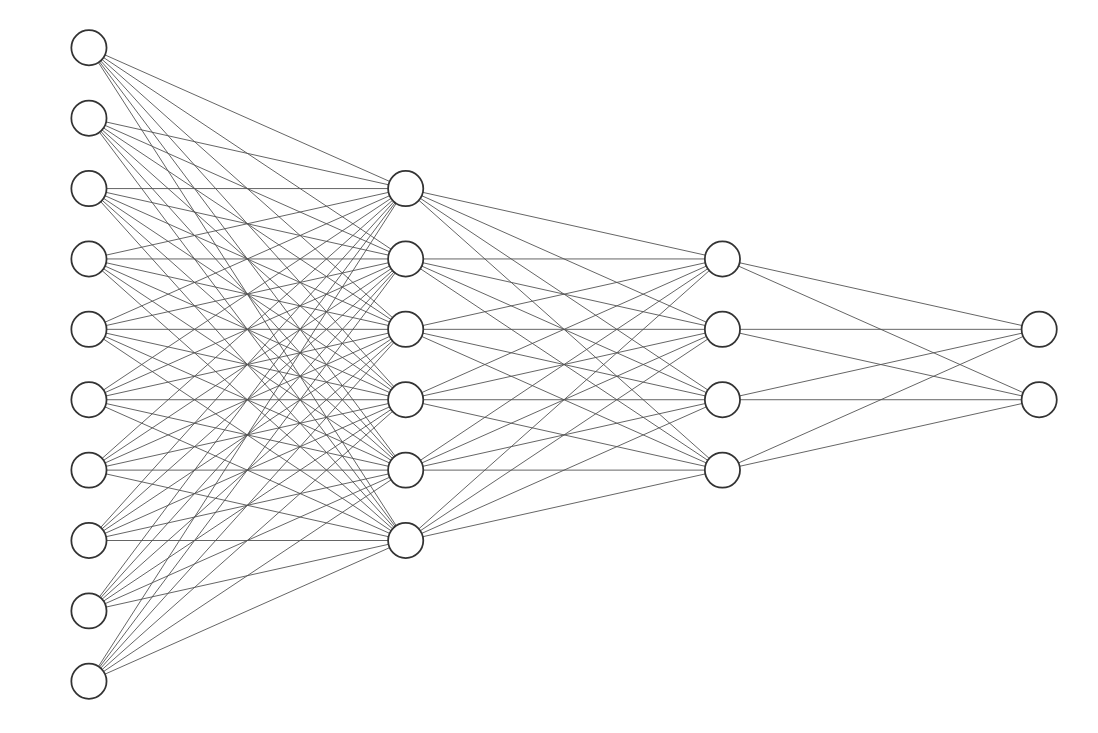
\includegraphics[width=1.0\linewidth]{imgs/emergent/nn1.png}
            \caption*{Parametri: 92}
        \end{figure}
    \end{column}
    
    \begin{column}{0.48\textwidth}
        \begin{figure}
            \centering
            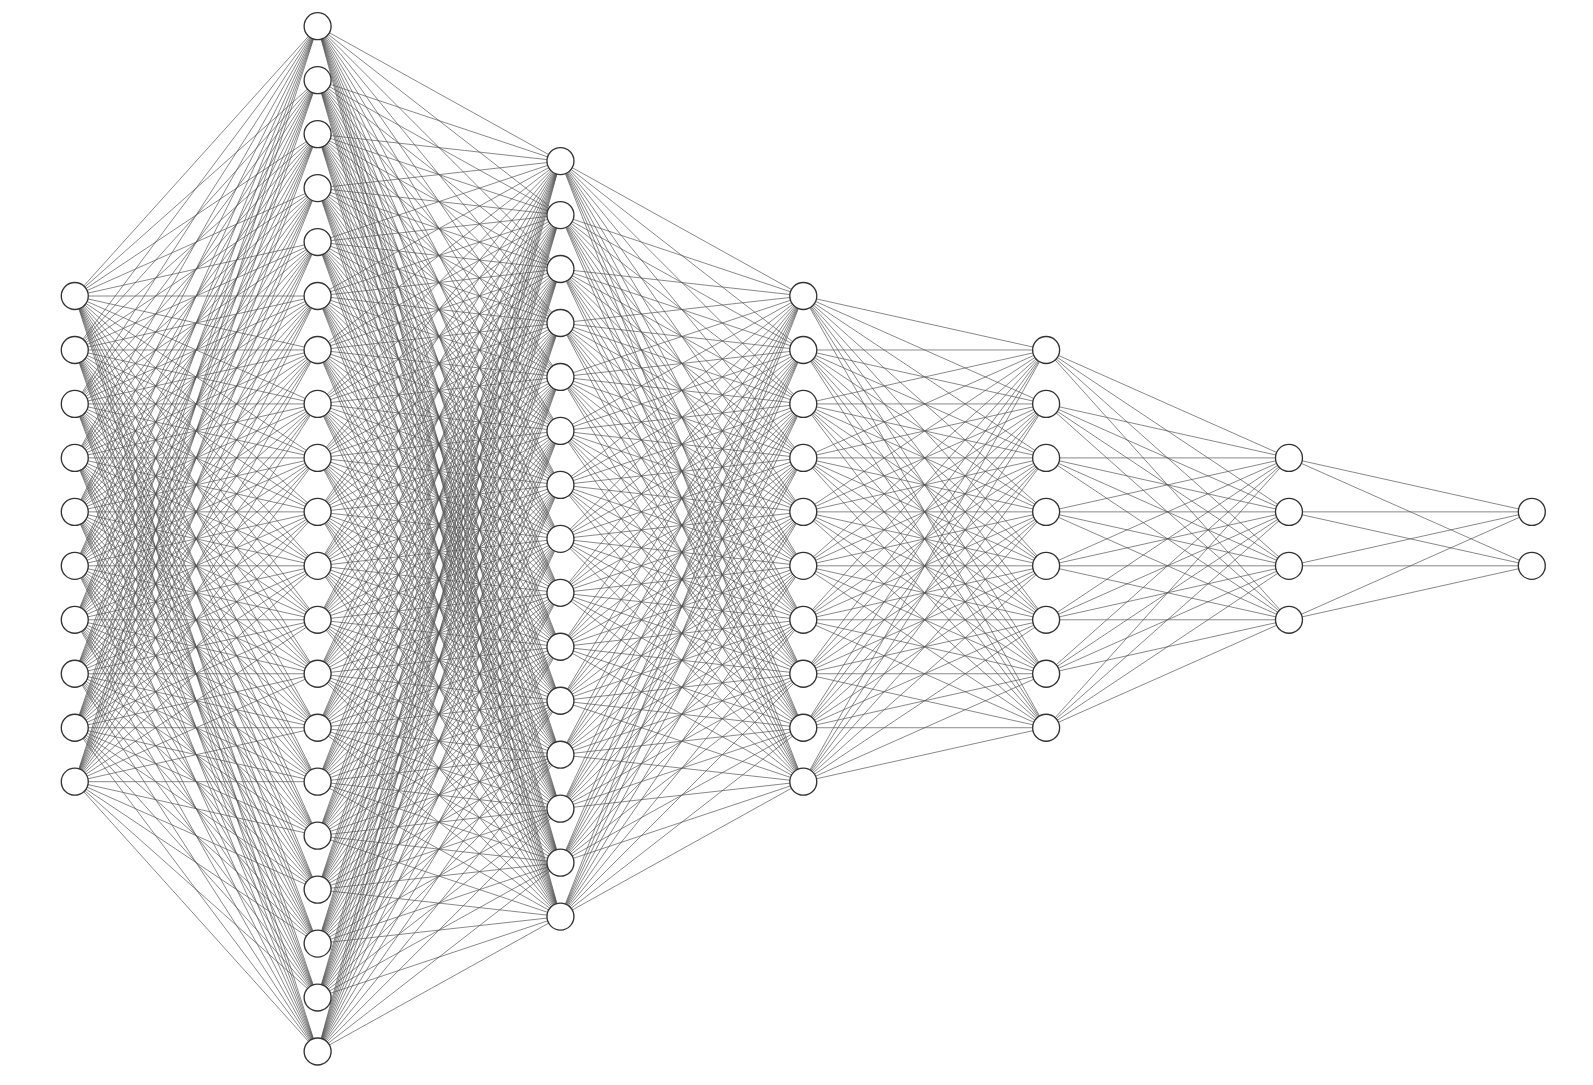
\includegraphics[width=1.0\linewidth]{imgs/emergent/nn2.png}
            \caption*{Parametri: 770}
        \end{figure}
    \end{column}
  \end{columns}
  \pause
  \begin{center}
    $\ldots$ ChatGPT 3: 175 Miliardi
  \end{center}
\end{frame}

\begin{frame}{Dimensioni dei modelli nel tempo}
    \begin{figure}
        \centering
        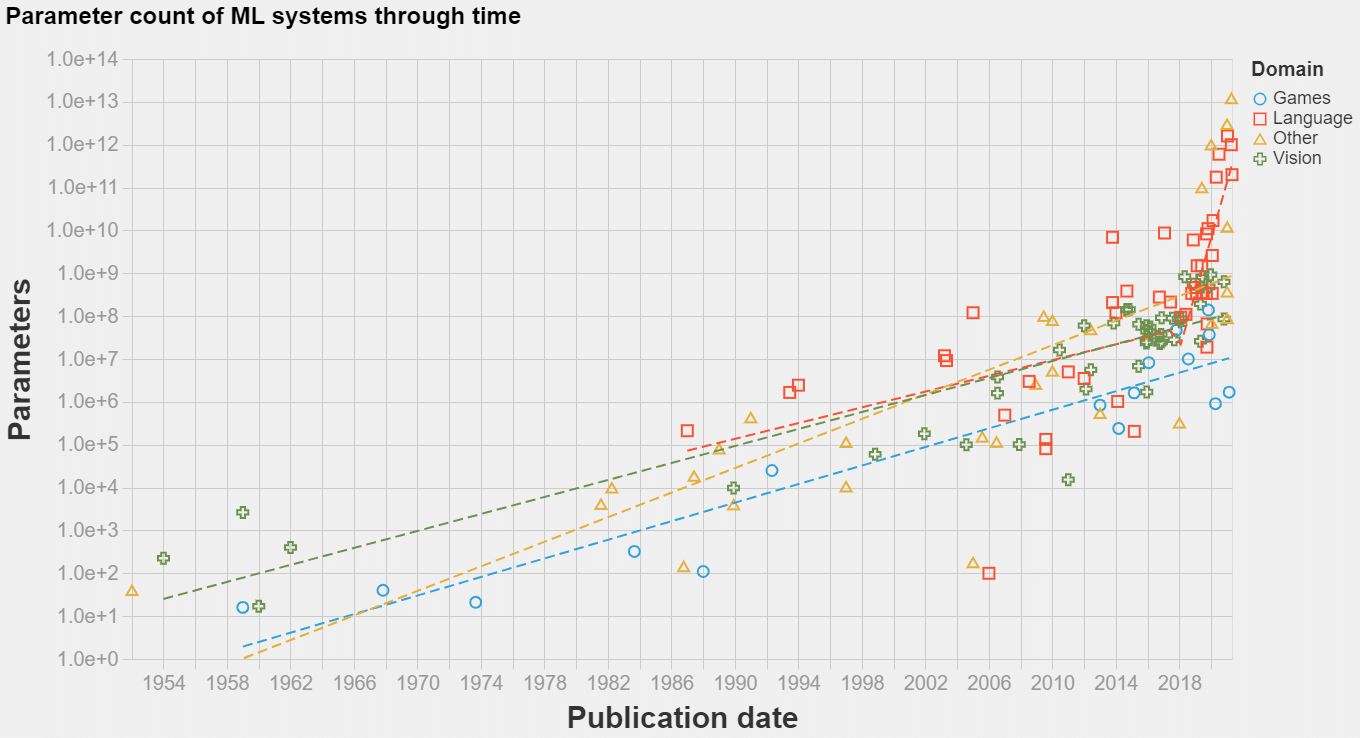
\includegraphics[width=0.9\linewidth]{imgs/emergent/nnsizes.png}
        \caption*{\tiny\textcolor{gray}{https://www.alignmentforum.org/}}
    \end{figure}
\end{frame}

\begin{frame}{Dimensioni dei modelli nel tempo}
    \begin{figure}
        \centering
        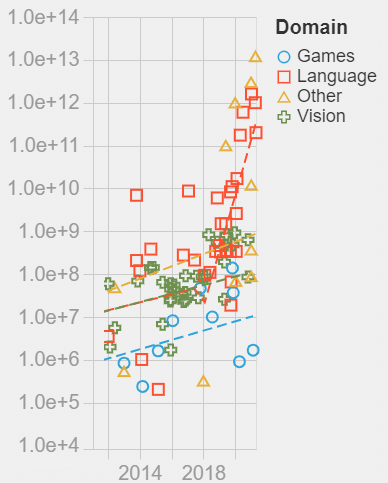
\includegraphics[width=0.5\linewidth]{imgs/emergent/nnzoom.png}
        \caption*{\tiny\textcolor{gray}{https://www.alignmentforum.org/}}
    \end{figure}
\end{frame}

    
\begin{frame}{Conclusioni}
    \begin{enumerate}
        \item \textbf{Quando nasce l'IA}: \pause  $~$ 1950, Alan Turing
        \pause
        \item \textbf{Come funziona ChatGPT}: \pause Generatore di Testo
        \pause
        \item \textbf{Stochastic Parrot}
        \pause
        \item \textbf{Comportamenti emergenti}: sintomo di intelligenza ?
    \end{enumerate}
\end{frame}

\begin{frame}[plain]
    \centering
    \vfill
    {\LARGE \textbf{Fine !}} \\[2em]

    \rule{0.5\linewidth}{0.4pt} \\[1em]
    
    \textbf{Nicolò Vescera} \\
    \texttt{nicolo.vescera@unifi.it} \\
    \href{https://github.com/ncvescera}{@ncvescera} \\
    \vfill
\end{frame}

\begin{frame}[allowframebreaks]{Bibliografia}
    \nocite{*}
    \printbibliography[heading=none]
\end{frame}
\end{document}